\chapter{Konzeption des Frameworks}
\label{chap:konzeption_pubsub}
Diese Arbeit entwickelt ein Framework auf Basis eines strukturierten P2P-Overlay-Netzwerkes. Die im System nutzbaren Publish/Subscribe-Systeme müssen ebenfalls verteilt arbeiten können. Dabei spielen die Fehlertoleranz und auch die Fähigkeit mit \emph{churn}, d.h. schnellem Wechsel der Mitgliedschaften, umgehen zu können, eine große Rolle.

\emph{Nicht vergessen}: Auf Knoten die Nachrichten weiterleiten wird \emph{forward} aufgerufen. Auf Knoten die eine Nachricht empfangen wird zuerst \emph{forward} und dann \emph{deliver} aufgerufen. In \emph{forward} kann der Knoten den Nachrichtenversand beenden. Vgl. \Fref{chap:evaluation_p2p:generic_api}!

Die Dimension \emph{Routing} entscheidet darüber ob und welche Nachrichten Typen in \emph{forward} oder \emph{deliver} behandelt werden sollen.\\
\emph{publish}-Nachrichten werden nicht in \emph{forward} sondern nur in \emph{deliver} behandelt.

Die Dimension \emph{Filter} muss sicherstellen, dass eine \emph{publish}-Nachricht nur an diejenigen Knoten geht, die diese Nachricht auch empfangen wollen. Muss eine solche Nachricht erst zum RootKnoten wandern (bsp. bei Direct oder Multicast) so, darf sie natürlich nicht gefiltert werden!\\
Dies bedeutet auch, dass bei der Auslieferung einer \emph{publish}-Nachricht nicht mehr gefiltert werden muss. Muss eine solche Nachricht jedoch weiter verteilt werden (bsp: Multicast), dann muss wie oben erwähnt gefiltert werden!


\cite{Fischer2010a, Fischer2010Event}


\cite{BeFiMu2006PubSubQoS}
\cite{KostasKatrinis2005}

\section{Problemstellung}

\section{Verarbeitungsmodell}
Dimensionen $\rightarrow$ Policies $\rightarrow$ Strategien

The processing model describes how the publish/subscribe system abstracts from the \ac{kbr} network, taking into consideration the different dimensions to optimize the event dissemination.

Each channel offers the common publish/subscribe actions: \emph{subscribe, unsubscribe} and \emph{publish}. Each action for each channel is connected with a corresponding type of message sent via the network. The network is accessed via a \ac{kbr}-API providing three methods to inform about new nodes joining the network, a message being forwarded and/or delivered to the user's node \cite{Dabek2003Towards}.

The semantical dimensions introduced in \cite{Fischer2010a} are covered by seven policies. These policies define the interfaces for the implementation of different strategies for each dimension and their implication on the processing of the publish/subscribe messages. We support following policies:
\\\textbf{Routing} is the logic of event dissemination and creates a multicast-tree. 
\\\textbf{Filter} permits to attach a filter predicate to subscribtions and ensures that these predicates are merged upwards in the multicast-tree to filter messages as early as possible.
\\\textbf{Delivery} defines the logic of the message delivery, e.g. acknowledgements.
\\\textbf{Order} defines the synchronization strategy for a channel.
\\\textbf{Persistence} provides persistence for messages delivered to the target nodes.
\\\textbf{Security} may be used to encrypt a channel.
\\\textbf{Validity} discards invalid messages and therefore decrease the amount of messages.

The mapping between publish/subscribe and \ac{kbr} actions is straight forward as table \ref{tab:verbindungsmatrix} shows. All policies are involved in the delivery of publish messages. This ensures that these messages arrive at the destination host and are not changed while routing. Subscribe and unsubscribe messages require actions in forward and deliver for routing and filtering purposes, as the decision of their strategies may affect the structure of the multicast-tree.

\begin{table}[!h]
\resizebox{\textwidth}{!}{%
\begin{tabular}{llccccccc}
\toprule
Nachrichten- & KBR	& \multicolumn{7}{c}{Policy für jeden Kanal} \\
\cmidrule{3-9}
typ				&	Aufruf	& Routing & Filter & Delivery & Order & Persistence & Security & Validity \\
\midrule
publish	    & deliver & + & + & + & + & + & + & + \\
\midrule
subscribe	  & deliver & + & + &   &   &   & + & \\
\cmidrule{2-9}
			      & forward & + & + &   &   &   & + & \\
\midrule
unsubscribe & deliver & + & + &   &   &   & + & \\
\cmidrule{2-9}
      & forward & + & + &   &   &   & + & \\
\bottomrule
\end{tabular}}
\caption{Verbindungsmatrix}
\label{tab:verbindungsmatrix}
\end{table}


Based on the given mapping, the challenge is to find a generic application order for the policies in the processing model as shown in figure \ref{fig:processing_model}.

For the distribution of a message the routing policy has to provide a list of target nodes, to whom the message must be send. Every multicast-tree has one or more corresponding root nodes. Subscribe or unsubscribe messages are always sent to that nodes, while publish messages from a non-root node must always be sent to the root nodes to trigger the publish process. Such messages are flagged \emph{to root}. On the root nodes, this flag is set to \emph{from root}. Nodes sending messages as \emph{from root} return the list of subscribers as target nodes which are filtered according to their predicate given at subscription. Finally the message is encrypted and handed over to the network.



\begin{figure}[htbp]
\centering
\resizebox{\textwidth}{!}{%
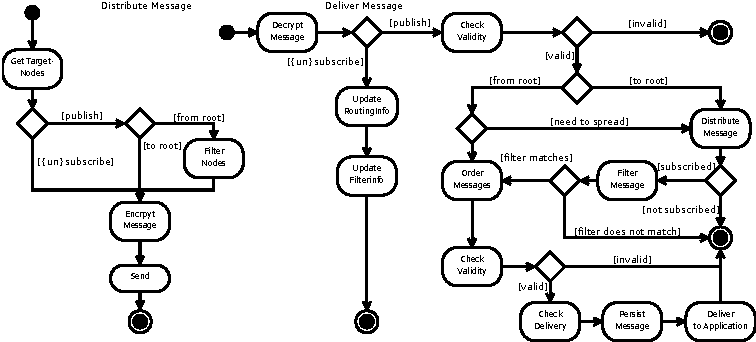
\includegraphics{grafics/processing_model.pdf}}
\caption{Verarbeitungsmodell}
\label{fig:processing_model}
\end{figure}

Decryption is the first action if a message is processed in deliver. After that subscribe and unsubscribe messages are handled separately. These messages are passed to the strategies for routing and filter to alter the multicast tree. Publish messages on the other hand have to pass the validity check. The next step checks whether the message must be spread i.e. distributed to other nodes. That is the case if the actual node is a root node or an intermediate node with distribution responsibility. If yes, the message is distributed using the send-process explained above. Now, the subscription and the predicate of the actual node are checked to ensure a proper delivery if that node is subscribed, too. If the actual node is a simple subscriber and the message is flagged \emph{from root} the predicate is not tested, as it is already checked while sending the message at the publishers side. The two paths merge at the ordering step. As ordering may hold messages back until they are ready the validity has to be checked again. The deliver dimension is called next offering to send acknowledgements back to the sender. Persisting the message is the last action before the message is finally delivered up to the application.\\
The handling in the forward-action from the \ac{kbr} is similar to deliver as the subscribe or unsubscribe information is extracted and passed to the strategies and they may alter the message.

As failures are not detected activeley in such networks, it is important to automatically renew the subscription. If nodes in the logical multicast-tree fail, the messages are automatically routed via other hosts, rebuilding the tree. However, it is possible that some messages are lost during the recovery.

\subsection{Beispielhafte Strategien}
For every policy \ac{m2etis} provides one ore more implementations. For example \emph{Direct} or \emph{Multicast} for routing. The framwork permits inclusion of more user-defined strategies. Different types of channel use a different set of implementations for every policy, creating a variety of optimization options. Each implemented strategy must provide additional cost information that is used in the optimizing step and they may add information onto each message to enable the customized treatment.

Using the example of Scribe \cite{Castro2002Scribe} and VON \cite{Hu2006VON} some details and inner workings of the processing model showed in figure \ref{fig:deliver} are explained. Scribe creates a multicast-tree trying to minimize the amount of messages while an algorithm like VON is neighborhood centric.

Using a scribe-like algorithm for routing \emph{Get Targetnodes} returns either the calculated root node for the channel or the list of subscribed nodes to which a publication must be forwarded. On the other hand a routing strategy like VON returns the in-game neighbors, obtained through application-level knowledge, as each node subscribes at his neighbors in the virtual world. Publications are sent to self enabling the distribution in deliver.

Scribe processes unsubscribe and subscribe messages in forward. Each node on the routing path adds the sender to its list of subscribers and can changes the message to create the multicast-tree. The periodic resubscription is triggerd externally for subscribed nodes as the channel will call its own subscribe method again or internally for intermediate routing hops as the algorithm will resend its subscriptions if other nodes down in the multicast-tree will refresh their subscribtion. It is necessary that the filter strategy is always involved to ensure the correct merge of predicates upwards the logical mulitcast-tree.

VON on the other hand does not need automatic periodic subscriptions, because each node will unsubscribe and subscribe frequently. Using the example of position updates it is obvious that each node and its neighbors move often and need to alter their subscribtions each frame in the game.

Using TTL or a timestamp-based approach for the strategy implementing the validity policy, the TTL would be increased on every routing hop or the passed time since the message was created is tested against the interval set in the strategy.

This exemplary discussion of different strategies indicates the generic nature of our processing model in terms of a multidimensional optimization for publish/subscribe channels.
